%%%%%%%%%%%%%%%%%%%%%%%%%%%%%%%%%%%%%%%%%%%%%%%%%%%
%                                                 %
%                     SECTION                     %
%                                                 %
%%%%%%%%%%%%%%%%%%%%%%%%%%%%%%%%%%%%%%%%%%%%%%%%%%%

\section*{Details}

Several modalities \cite{kopans2004breast} are used as an adjunct look modality for questionable situations where the breast of the patient has a life time risk. The images produced by the \textbf{Medical Imaging (MI)} exams are similar in acquisition, however the costs (time and money) are typically different. This behaviour is leading the \textbf{RR} workflow standards and methodology to remain scarce \cite{rawson2016lessons, saltzherr2013cost}, which give us little information to support a workflow validation through interviews and observations. Therefore, we will not assume a low-level workflow of the \textbf{RR} and will assume from now a high-level workflow, where the rules to trigger the acquisition of the several modalities are not specified.

\hfill

The following text can be used to motivate/introduce a final paper to write. So it's more or less like this:

%%%%%%%%%%%%%%%%%%%%%%%%%%%%%%%%%%%%%%%%%%%%%%%%%%%

\hfill

\begin{enumerate}

\item Mammography appears as the 1st imaging modality, and constitutes a screening exam. The reason is that the exam in this modality (X-Ray) has little cost.

\item It is begun to realise that not all the examinations (recognised) in mammography are conclusive. The main reason for this is the type of breast (Figure \ref{fig:workflow}). There are two types \cite{nothacker2009early, rhodes2011dedicated} of breasts: (1) adipose breasts (patterns A and B) and (2) dense breasts (patterns C and D). These types are leaving an international standard where mammography may not be sufficient in the diagnosis of a dense breast by concluding that this type of chest is opaque to the X-Ray. According to study was done, the dense breasts have 2X or 4X more likely to develop a tumour than the adipose breast.

\hfill

\textbf{Note:} supporting this international standard by the fact that there were cases where women unexpectedly possessed advanced tumours, although they did frequent X-Ray screenings.

\hfill

\item Therefore, it is necessary to have an additional examination, particularly in case of dense breast, in standards C and D (Figure \ref{fig:workflow}). Doing in these cases an ultrasound.

%%%%%%%%%%%%%%%%%%%%%%%%%%%%%%%%%%%%%%%%%%%%%%%%%%%

\hfill

\begin{figure}[h]
\centering
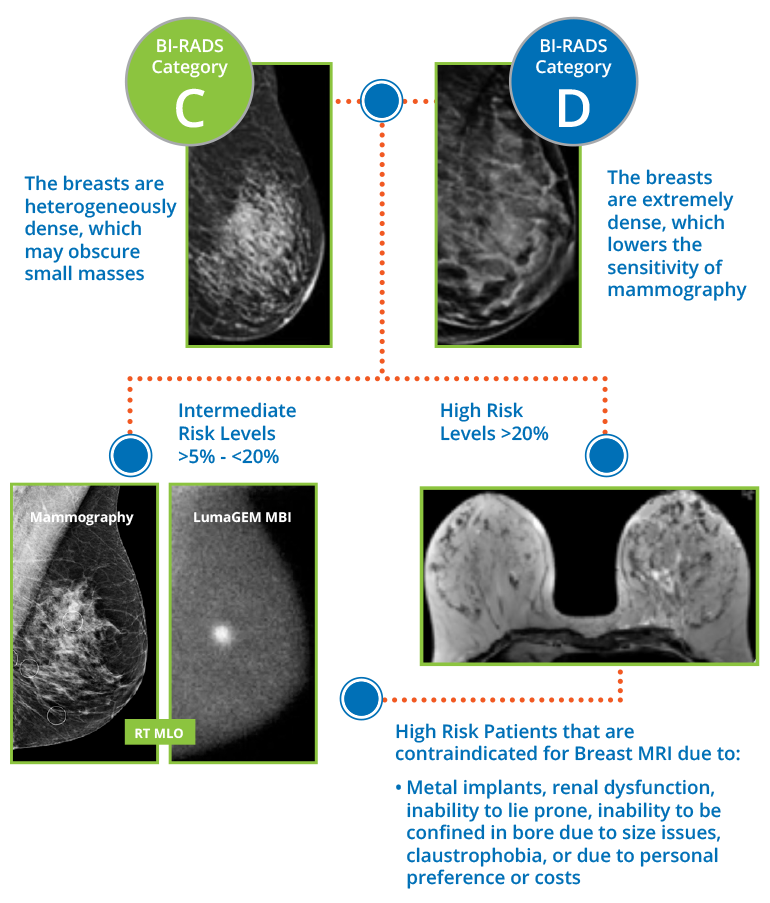
\includegraphics[width=0.50\textwidth]{workflow}
\caption{Dense Breast Workflow \cite{workflow} for C and D Standards}
\label{fig:workflow}
\end{figure}

\hfill

%%%%%%%%%%%%%%%%%%%%%%%%%%%%%%%%%%%%%%%%%%%%%%%%%%%

\item There is not yet an international guideline (or standards) for elaborating MRI (which is a very expensive kind of exam). We proceed to this type of examination for women with family risk, the so-called BRCA1 and BRCA2 \cite{chen2007meta}. Being these mutations that the woman suffers, and being able to provoke a tumour (the case, for example, of Angelina Jolie).

\item In other cases (not mentioned in point 4) it is up to the radiologist to do MRI or not. It can happen, for instance, that on the palpation (performed by the radiologist) there are indications of tumour presence, without any suspicion in mammography. There you will advance to the MRI.

\item Still about point 5, there are cases where the patient is followed, and calcifications with suspected morphology are recorded (in mammography). In these situations, the radiologist advances to MRI.

\end{enumerate}

\hfill

%%%%%%%%%%%%%%%%%%%%%%%%%%%%%%%%%%%%%%%%%%%%%%%%%%%

Despite of not having a standard \textbf{MI} acquisition workflow we can informally map the information workflow of the \textbf{RR}. On Figure \ref{fig:rr_workflow} we cover the steps of the clinical workflow including treatment planning (\textit{Referring}), information control (\textit{Study Order}), stored data (\textit{Medical Imaging Studies} and \textit{Image Stored}), data retrieval (\textit{Retrieved Information}), image analysis (\textit{Modality Worklist}) and diagnosis (\textit{Report}).

%%%%%%%%%%%%%%%%%%%%%%%%%%%%%%%%%%%%%%%%%%%%%%%%%%%

\hfill

\begin{figure}[h]
\centering
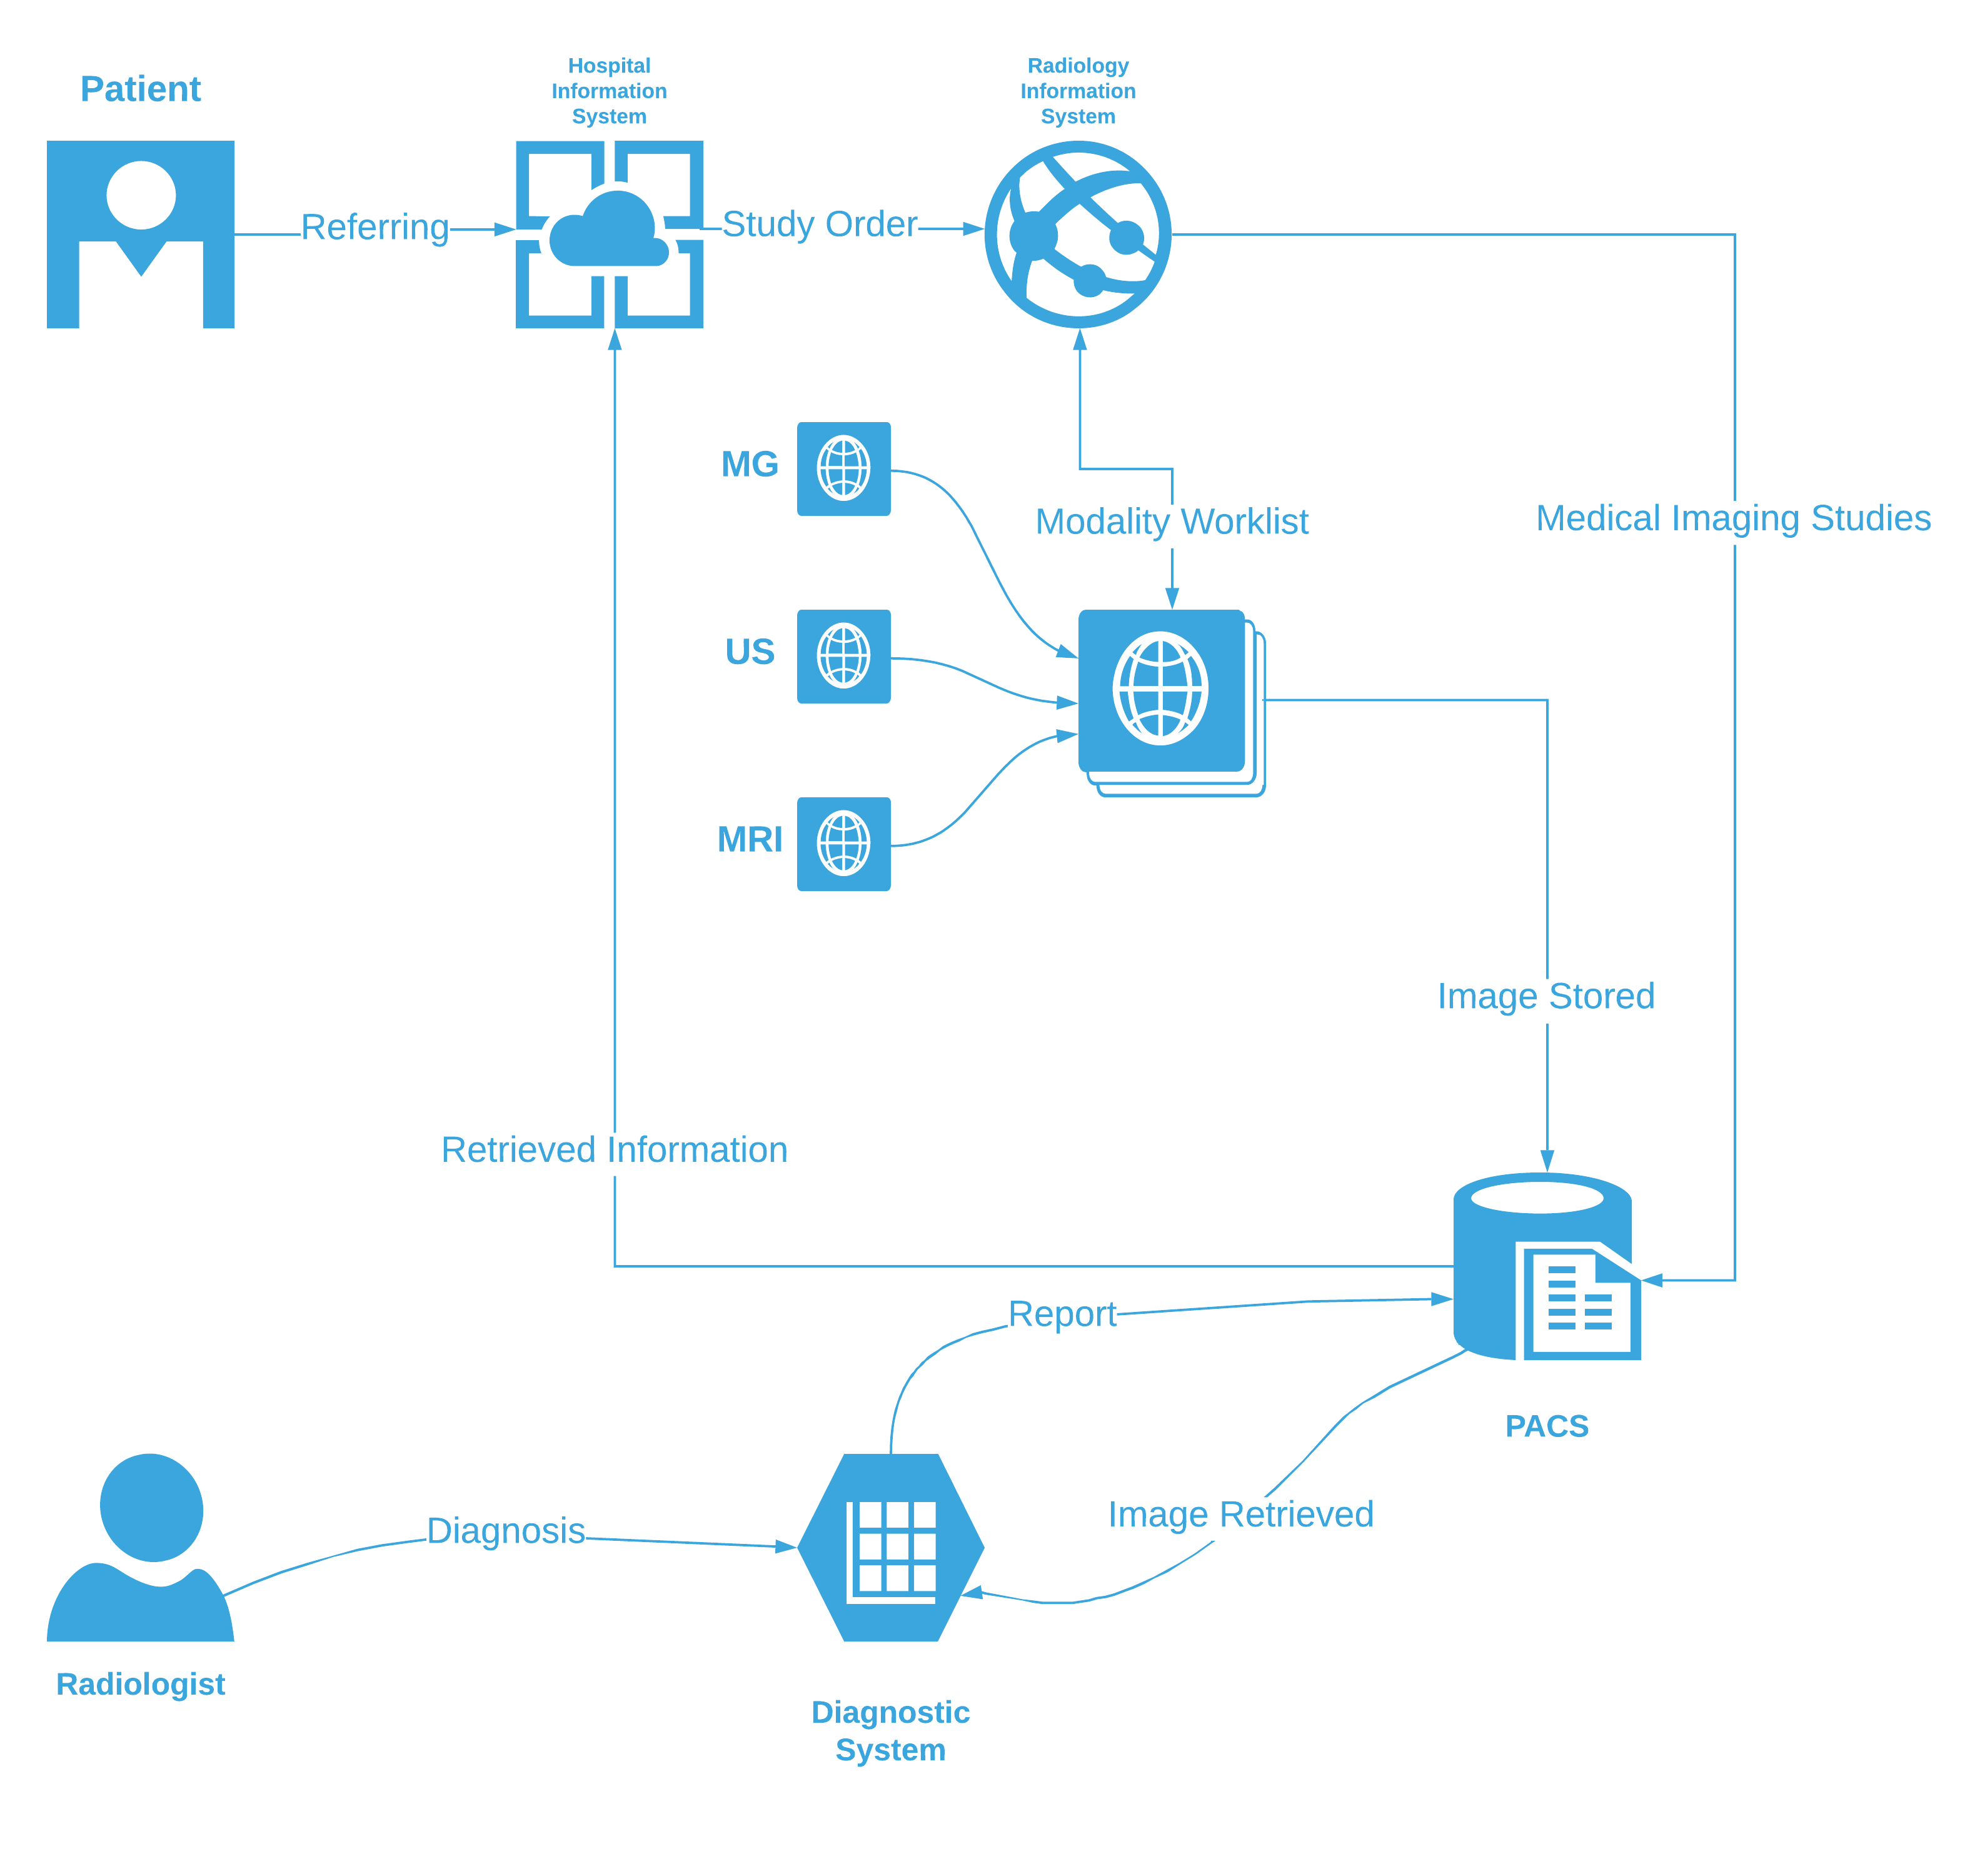
\includegraphics[width=0.75\textwidth]{rr_workflow}
\caption{Radiology Room Workflow}
\label{fig:rr_workflow}
\end{figure}

\hfill

%%%%%%%%%%%%%%%%%%%%%%%%%%%%%%%%%%%%%%%%%%%%%%%%%%%

To start the description of what we observed to be the information workflow of the \textbf{RR}, first of all, a \textit{Patient} is \textit{Referred} to a \textit{Hospital Information System (HIS)}. From this step, a \textit{Study Order} is created and received by a \textit{Radiology Information System (RIS)}. The \textit{RIS} can do two things: (1) it can receive the \textit{Modality Worklist} (e.g. \textit{MG}, \textit{US} or \textit{MRI}) and store it (\textit{Image Stored}) on the \textit{PACS}; and (2) it can access the \textit{Medical Imaging Studies}. From here, the \textit{HIS} can also retrieve  information (\textit{Retrieved Information}) from the \textit{PACS}. Finally, the \textit{Radiologist} do the respective \textit{Diagnosis} of the \textit{Patient} through a \textit{Diagnostic System} and \textit{Report} it to the \textit{PACS}.

%%%%%%%%%%%%%%%%%%%%%%%%%%%%%%%%%%%%%%%%%%%%%%%%%%%